\newcommand{\titulus}{\nomenFesti{S. Callisti I, Papæ \& Martyris.}
\dies{Die 14. Octobris.}}
\newcommand{\sineobmv}{Sine officium B.M.V.}
\newcommand{\oratio}{\pars{Oratio.}

\noindent Preces pópuli tui, quǽsumus, Dómine, cleménter exáudi, ut beáti Callísti, papæ, méritis adiuvémur, cuius passióne lætámur.

\pars{Pro pace in Ucraina.} \scriptura{Sir. 50, 25; 2 Esdr. 4, 20; \textbf{H416}}

\vspace{-4mm}

\antiphona{II D}{temporalia/ant-dapacemdomine.gtex}

\vfill

\noindent Deus, a quo sancta desidéria, recta consília et iusta sunt ópera: da servis tuis illam, quam mundus dare non potest, pacem; ut et corda nostra mandátis tuis dédita, et hóstium subláta formídine, témpora sint tua protectióne tranquílla.

\noindent Per Dóminum nostrum Iesum Christum, Fílium tuum, qui tecum vivit et regnat in unitáte Spíritus Sancti, Deus, per ómnia sǽcula sæculórum.

\noindent \Rbardot{} Amen.}
\newcommand{\invitatorium}{\pars{Invitatorium.}

\vspace{-4mm}

\antiphona{E}{temporalia/inv-regemmartyrumsimplex.gtex}}
\newcommand{\hymnusmatutinum}{\pars{Hymnus}

\cuminitiali{I}{temporalia/hym-BeateMartyr.gtex}}
\newcommand{\matversus}{\noindent \Vbardot{} Fili mi, atténde ad sapiéntiam meam.

\noindent \Rbardot{} Et prudéntiæ meæ inclína aurem tuam.}
\newcommand{\lectioi}{\pars{Lectio I.} \scriptura{1 Tim. 6, 11-21}

\noindent De Epístola prima beáti Pauli apóstoli ad Timótheum.

\noindent Tu, o homo Dei, hæc fuge; sectáre vero iustítiam, pietátem, fidem, caritátem, patiéntiam, mansuetúdinem. Certa bonum certámen fídei, apprehénde vitam ætérnam, ad quam vocátus es, et conféssus es bonam confessiónem coram multis téstibus.

\noindent Præcípio tibi coram Deo, qui vivíficat ómnia, et Christo Iesu, qui testimónium réddidit sub Póntio Piláto bonam confessiónem, ut serves mandátum sine mácula irreprehensíbile usque in advéntum Dómini nostri Iesu Christi, quem suis tempóribus osténdet beátus et solus potens, Rex regnántium et Dóminus dominántium, qui solus habet immortalitátem, lucem hábitans inaccessíbilem, quem vidit nullus hóminum nec vidére potest; cui honor et impérium sempitérnum. Amen.

\noindent Divítibus huius sǽculi prǽcipe non supérbe sápere neque speráre in incérto divitiárum, sed in Deo, qui præstat nobis ómnia abúnde ad fruéndum, bene ágere, dívites fíeri in opéribus bonis, fácile tribúere, communicáre, thesaurizáre sibi fundaméntum bonum in futúrum, ut apprehéndant veram vitam.

\noindent O Timóthee, depósitum custódi, devítans profánas vocum novitátes et oppositiónes falsi nóminis sciéntiæ, quam quidam profiténtes circa fidem aberravérunt.

\noindent Grátia vobíscum.}
\newcommand{\responsoriumi}{\pars{Responsorium 1.} \scriptura{\Rbardot{} Ps. 100, 1-2 \Vbardot{} ibid., 2; \textbf{H89}}

\vspace{-5mm}

\responsorium{III}{temporalia/resp-misericordiametiudicium-CROCHU.gtex}{}}
\newcommand{\lectioii}{\pars{Lectio II.} \scriptura{Cap. 13: CSEL 3, 346-347}

\noindent Ex Tractátu sancti Cypriáni epíscopi et mártyris ad Fortunátum.

\noindent \emph{Non sunt condígnæ passiónes huius témporis ad superventúram claritúdinem quæ revelábitur in nobis.} Quis ergo non ómnibus modis elabóret ad claritátem tantam perveníre, ut amícus Dei fiat, ut cum Christo statim gáudeat, ut post torménta et supplícia terréna prǽmia divína percípiat? Si milítibus sæculáribus gloriósum est ut hoste devícto rédeant in pátriam triumphántes, quanto pótior et maior est glória victo diábolo ad paradísum triumphántem redíre et, unde Adam peccátor eiéctus est, illuc prostráto eo qui ante decéperat tropǽa victrícia reportáre, offérre Dómino acceptíssimum munus incorrúptam fidem, virtútem mentis incólumem, laudem devotiónis illústrem, comitári eum cum veníre cœ́perit vindíctam de inimícis receptúrus, láteri eius assístere cum séderit iudicatúrus, coherédem Christi fíeri, ángelis coæquári, cum patriárchis, cum apóstolis, cum prophétis cæléstis regni possessióne lætári.}
\newcommand{\responsoriumii}{\pars{Responsorium 2.} \scriptura{\textbf{H373}}

\vspace{-5mm}

\responsorium{III}{temporalia/resp-istecognovit-CROCHU.gtex}{}

\vfill
\pagebreak

\rubrica{vel ad libitum:}

\vspace{3mm}

\pars{Responsorium 2.}

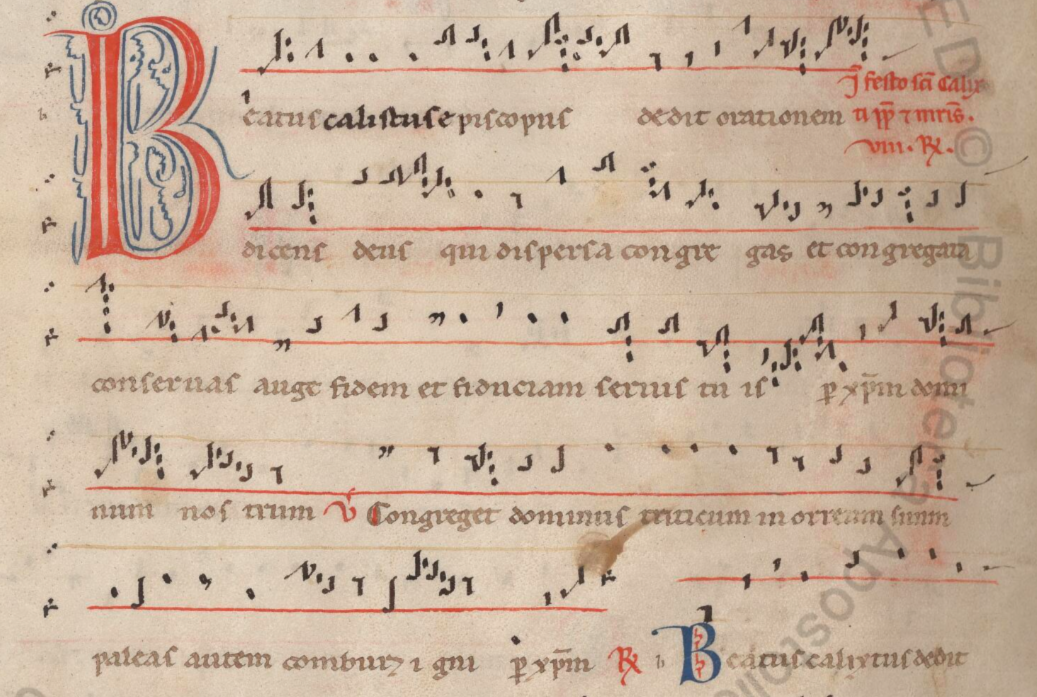
\includegraphics[width=17cm]{pic-beatuscallistus.png}}
\newcommand{\lectioiii}{\pars{Lectio III.}

\noindent Has cogitatiónes quæ persecútio potest víncere, quæ possunt torménta superáre? Durat fortis et stábilis religiósis meditatiónibus fundáta mens et advérsus omnes diáboli terróres et minas mundi ánimus immóbilis perstat, quem futurórum fides certa et sólida corróborat. Claudúntur in persecutiónibus terræ, sed patet cælum; minátur antichrístus, sed Christus tuétur; mors infértur, sed immortálitas séquitur. Quanta est dígnitas et quanta secúritas exíre hinc lætum, exíre inter pressúras et angústias gloriósum, cláudere in moménto óculos, quibus hómines videbántur et mundus, aperíre eósdem statim, ut Deus videátur et Christus. Tam felíciter migrándi quanta velócitas. Terris repénte subtráheris, ut in regnis cæléstibus reponáris.

\noindent Hæc opórtet mente et cogitatióne complécti, hæc die ac nocte meditári. Si talem persecútio invénerit Dei mílitem, vinci non póterit virtus ad prœ́lium prompta. Vel si arcessítio ante prævénerit, sine prǽmio non erit fides quæ erat ad martýrium præparáta; sine damno témporis merces Deo iúdice rédditur; in persecutióne milítia, in pace consciéntia coronátur.}
\newcommand{\responsoriumiii}{\pars{Responsorium 3.} \scriptura{\Rbardot{} Ps. 8, 6-8 \Vbardot{} Ps. 20, 4; \textbf{H374}}

\vspace{-5mm}

\responsorium{VII}{temporalia/resp-gloriaethonore-CROCHU-cumdox.gtex}{}}
\newcommand{\hymnuslaudes}{\pars{Hymnus}

\cuminitiali{VI}{temporalia/hym-MartyrDei.gtex}}
\newcommand{\lectiobrevis}{\pars{Lectio Brevis.} \scriptura{2 Cor. 1, 3-5}

\noindent Benedíctus Deus et Pater Dómini nostri Iesu Christi, Pater misericordiárum et Deus totíus consolatiónis, qui consolátur nos in omni tribulatióne nostra, ut possímus et ipsi consolári eos, qui in omni pressúra sunt, per exhortatiónem, qua exhortámur et ipsi a Deo; quóniam, sicut abúndant passiónes Christi in nobis, ita per Christum abúndat et consolátio.}
\newcommand{\responsoriumbreve}{\pars{Responsorium breve.} \scriptura{Ex. 15, 2}

\cuminitiali{VI}{temporalia/resp-fortitudomeaetlausmea.gtex}}
\newcommand{\preces}{\noindent Fratres, Salvatórem nostrum, testem fidélem, per mártyres interféctos propter verbum Dei,~\gredagger{} celebrémus, clamántes:

\Rbardot{} Redemísti nos Deo in sánguine tuo.

\noindent Per mártyres tuos, qui líbere mortem in testimónium fídei sunt ampléxi,~\gredagger{} da nobis, Dómine, veram spíritus libertátem.

\Rbardot{} Redemísti nos Deo in sánguine tuo.

\noindent Per mártyres tuos, qui fidem usque ad sánguinem sunt conféssi,~\gredagger{} da nobis, Dómine, puritátem fideíque constántiam.

\Rbardot{} Redemísti nos Deo in sánguine tuo.

\noindent Per mártyres tuos, qui, sustinéntes crucem, tua vestígia sunt secúti,~\gredagger{} da nobis, Dómine, ærúmnas vitæ fórtiter sustinére.

\Rbardot{} Redemísti nos Deo in sánguine tuo.

\noindent Per mártyres tuos, qui stolas suas lavérunt in sánguine Agni,~\gredagger{} da nobis, Dómine, omnes insídias carnis mundíque devíncere.

\Rbardot{} Redemísti nos Deo in sánguine tuo.}
\newcommand{\benedictus}{\pars{Canticum Zachariæ.} \scriptura{Io. 12, 35; \textbf{H375}}

\vspace{-4mm}

\antiphona{III a}{temporalia/ant-quisequiturmenonambulat.gtex}

%\vspace{-2mm}

\scriptura{Lc. 1, 68-79}

\vspace{-2mm}

\cantusSineNeumas
\initiumpsalmi{temporalia/benedictus-initium-iii-a-auto.gtex}

%\vspace{-1.5mm}

\input{temporalia/benedictus-iii-a.tex} \Abardot{}}
\newcommand{\benedicamuslaudes}{\cuminitiali{}{temporalia/benedicamus-memoria-laudes.gtex}}
\newcommand{\hebdomada}{infra Hebdom. XXIII per Annum.}
\newcommand{\hiemalis}{Hiemalis}
\newcommand{\matuc}{Matutinum Hebdomadae C}
\newcommand{\matuac}{Matutinum Hebdomadae A vel C}
\newcommand{\laudc}{Laudes Hebdomadae C}
\newcommand{\laudac}{Laudes Hebdomadae A vel C}

% LuaLaTeX

\documentclass[a4paper, twoside, 12pt]{article}
\usepackage[latin]{babel}
%\usepackage[landscape, left=3cm, right=1.5cm, top=2cm, bottom=1cm]{geometry} % okraje stranky
%\usepackage[landscape, a4paper, mag=1166, truedimen, left=2cm, right=1.5cm, top=1.6cm, bottom=0.95cm]{geometry} % okraje stranky
\usepackage[landscape, a4paper, mag=1400, truedimen, left=0.5cm, right=0.5cm, top=0.5cm, bottom=0.5cm]{geometry} % okraje stranky

\usepackage{fontspec}
\setmainfont[FeatureFile={junicode.fea}, Ligatures={Common, TeX}, RawFeature=+fixi]{Junicode}
%\setmainfont{Junicode}

% shortcut for Junicode without ligatures (for the Czech texts)
\newfontfamily\nlfont[FeatureFile={junicode.fea}, Ligatures={Common, TeX}, RawFeature=+fixi]{Junicode}

% Hebrew font:
% http://scripts.sil.org/cms/scripts/page.php?site_id=nrsi&id=SILHebrUnic2
\newfontfamily\hebfont[Scale=1]{Ezra SIL}

\usepackage{multicol}
\usepackage{color}
\usepackage{lettrine}
\usepackage{fancyhdr}

% usual packages loading:
\usepackage{luatextra}
\usepackage{graphicx} % support the \includegraphics command and options
\usepackage{gregoriotex} % for gregorio score inclusion
\usepackage{gregoriosyms}
\usepackage{wrapfig} % figures wrapped by the text
\usepackage{parcolumns}
\usepackage[contents={},opacity=1,scale=1,color=black]{background}
\usepackage{tikzpagenodes}
\usepackage{calc}
\usepackage{longtable}
\usetikzlibrary{calc}

\setlength{\headheight}{14.5pt}

% Commands used to produce a typical "Conventus" booklet

\newenvironment{titulusOfficii}{\begin{center}}{\end{center}}
\newcommand{\dies}[1]{#1

}
\newcommand{\nomenFesti}[1]{\textbf{\Large #1}

}
\newcommand{\celebratio}[1]{#1

}

\newcommand{\hora}[1]{%
\vspace{0.5cm}{\large \textbf{#1}}

\fancyhead[LE]{\thepage\ / #1}
\fancyhead[RO]{#1 / \thepage}
\addcontentsline{toc}{subsection}{#1}
}

% larger unit than a hora
\newcommand{\divisio}[1]{%
\begin{center}
{\Large \textsc{#1}}
\end{center}
\fancyhead[CO,CE]{#1}
\addcontentsline{toc}{section}{#1}
}

% a part of a hora, larger than pars
\newcommand{\subhora}[1]{
\begin{center}
{\large \textit{#1}}
\end{center}
%\fancyhead[CO,CE]{#1}
\addcontentsline{toc}{subsubsection}{#1}
}

% rubricated inline text
\newcommand{\rubricatum}[1]{\textit{#1}}

% standalone rubric
\newcommand{\rubrica}[1]{\vspace{3mm}\rubricatum{#1}}

\newcommand{\notitia}[1]{\textcolor{red}{#1}}

\newcommand{\scriptura}[1]{\hfill \small\textit{#1}}

\newcommand{\translatioCantus}[1]{\vspace{1mm}%
{\noindent\footnotesize \nlfont{#1}}}

% pruznejsi varianta nasledujiciho - umoznuje nastavit sirku sloupce
% s prekladem
\newcommand{\psalmusEtTranslatioB}[3]{
  \vspace{0.5cm}
  \begin{parcolumns}[colwidths={2=#3}, nofirstindent=true]{2}
    \colchunk{
      \input{#1}
    }

    \colchunk{
      \vspace{-0.5cm}
      {\footnotesize \nlfont
        \input{#2}
      }
    }
  \end{parcolumns}
}

\newcommand{\psalmusEtTranslatio}[2]{
  \psalmusEtTranslatioB{#1}{#2}{8.5cm}
}


\newcommand{\canticumMagnificatEtTranslatio}[1]{
  \psalmusEtTranslatioB{#1}{temporalia/extra-adventum-vespers/magnificat-boh.tex}{12cm}
}
\newcommand{\canticumBenedictusEtTranslatio}[1]{
  \psalmusEtTranslatioB{#1}{temporalia/extra-adventum-laudes/benedictus-boh.tex}{10.5cm}
}

% volne misto nad antifonami, kam si zpevaci dokresli neumy
\newcommand{\hicSuntNeumae}{\vspace{0.5cm}}

% prepinani mista mezi notovymi osnovami: pro neumovane a neneumovane zpevy
\newcommand{\cantusCumNeumis}{
  \setgrefactor{17}
  \global\advance\grespaceabovelines by 5mm%
}
\newcommand{\cantusSineNeumas}{
  \setgrefactor{17}
  \global\advance\grespaceabovelines by -5mm%
}

% znaky k umisteni nad inicialu zpevu
\newcommand{\superInitialam}[1]{\gresetfirstlineaboveinitial{\small {\textbf{#1}}}{\small {\textbf{#1}}}}

% pars officii, i.e. "oratio", ...
\newcommand{\pars}[1]{\textbf{#1}}

\newenvironment{psalmus}{
  \setlength{\parindent}{0pt}
  \setlength{\parskip}{5pt}
}{
  \setlength{\parindent}{10pt}
  \setlength{\parskip}{10pt}
}

%%%% Prejmenovat na latinske:
\newcommand{\nadpisZalmu}[1]{
  \hspace{2cm}\textbf{#1}\vspace{2mm}%
  \nopagebreak%

}

% mode, score, translation
\newcommand{\antiphona}[3]{%
\hicSuntNeumae
\superInitialam{#1}
\includescore{#2}

#3
}
 % Often used macros

\newcommand{\annusEditionis}{2021}

\def\hebinitial#1{%
\leavevmode{\newbox\hebbox\setbox\hebbox\hbox{\hebfont{#1}\hskip 1mm}\kern -\wd\hebbox\hbox{\hebfont{#1}\hskip 1mm}}%
}

%%%% Vicekrat opakovane kousky

\newcommand{\anteOrationem}{
  \rubrica{Ante Orationem, cantatur a Superiore:}

  \pars{Supplicatio Litaniæ.}

  \cuminitiali{}{temporalia/supplicatiolitaniae.gtex}

  \pars{Oratio Dominica.}

  \cuminitiali{}{temporalia/oratiodominica.gtex}
}

\setlength{\columnsep}{30pt} % prostor mezi sloupci

%%%%%%%%%%%%%%%%%%%%%%%%%%%%%%%%%%%%%%%%%%%%%%%%%%%%%%%%%%%%%%%%%%%%%%%%%%%%%%%%%%%%%%%%%%%%%%%%%%%%%%%%%%%%%
\begin{document}

% Here we set the space around the initial.
% Please report to http://home.gna.org/gregorio/gregoriotex/details for more details and options
\grechangedim{afterinitialshift}{2.2mm}{scalable}
\grechangedim{beforeinitialshift}{2.2mm}{scalable}

\grechangedim{interwordspacetext}{0.22 cm plus 0.15 cm minus 0.05 cm}{scalable}%
\grechangedim{annotationraise}{-0.2cm}{scalable}

% Here we set the initial font. Change 38 if you want a bigger initial.
% Emit the initials in red.
\grechangestyle{initial}{\color{red}\fontsize{38}{38}\selectfont}

\pagestyle{empty}

%%%% Titulni stranka
\begin{titulusOfficii}
\ifx\titulus\undefined
\nomenFesti{Sabbato \hebdomada{}}
\else
\titulus
\fi
\end{titulusOfficii}

\vfill

\pars{}

\scriptura{}

\pagebreak

% graphic
\renewcommand{\headrulewidth}{0pt} % no horiz. rule at the header
\fancyhf{}
\pagestyle{fancy}

\cantusSineNeumas

\hora{Ad Matutinum.}

\vspace{2mm}

\cuminitiali{}{temporalia/dominelabiamea.gtex}

\vspace{2mm}

\ifx\invitatorium\undefined
\pars{Invitatorium.} \scriptura{\textbf{H14}}

\vspace{-6mm}

\antiphona{VI}{temporalia/inv-regemventurumsimplex.gtex}
\else
\invitatorium
\fi

\vfill
\pagebreak

\ifx\hymnusmatutinum\undefined
\pars{Hymnus.}

\vspace{-5mm}

\antiphona{II}{temporalia/hym-VerbumSupernum.gtex}
\else
\hymnusmatutinum
\fi

\vfill
\pagebreak

\ifx\matutinum\undefined
\ifx\matua\undefined
\else
% MAT A
\pars{Psalmus 1.} \scriptura{Ps. 104, 3; \textbf{H99}}

\vspace{-6mm}

\antiphona{D}{temporalia/ant-laeteturcor.gtex}

\vspace{-4mm}

\scriptura{Ps. 104, 1-15}

\vspace{-2mm}

\initiumpsalmi{temporalia/ps104i-initium-d-g-auto.gtex}

\vspace{-1.5mm}

\input{temporalia/ps104i-d-g.tex} \Abardot{}

\vfill
\pagebreak

\pars{Psalmus 2.} \scriptura{Ps. 113, 1; \textbf{H94}}

\vspace{-4mm}

\antiphona{VIII a}{temporalia/ant-domusiacob.gtex}

%\vspace{-2mm}

\scriptura{Ps. 104, 16-27}

%\vspace{-2mm}

\initiumpsalmi{temporalia/ps104ii-initium-viii-a-auto.gtex}

\input{temporalia/ps104ii-viii-a.tex} \Abardot{}

\vfill
\pagebreak

\pars{Psalmus 3.} \scriptura{Ps. 104, 43}

\vspace{-4mm}

\antiphona{IV E}{temporalia/ant-eduxitdeus.gtex}

%\vspace{-2mm}

\scriptura{Ps. 104, 28-45}

%\vspace{-2mm}

\initiumpsalmi{temporalia/ps104iii-initium-iv-E-auto.gtex}

\input{temporalia/ps104iii-iv-E.tex}

\vfill

\antiphona{}{temporalia/ant-eduxitdeus.gtex}

\vfill
\pagebreak\fi
\ifx\matub\undefined
\else
% MAT B
\pars{Psalmus 1.} \scriptura{Ps. 105, 4; \textbf{H100}}

\vspace{-4mm}

\antiphona{E}{temporalia/ant-visitanos.gtex}

%\vspace{-2mm}

\scriptura{Ps. 105, 1-15}

%\vspace{-2mm}

\initiumpsalmi{temporalia/ps105i-initium-e.gtex}

\input{temporalia/ps105i-e.tex}

\vfill

\antiphona{}{temporalia/ant-visitanos.gtex}

\vfill
\pagebreak

\pars{Psalmus 2.} \scriptura{Ps. 117, 6; \textbf{H156}}

\vspace{-8mm}

\antiphona{VIII G}{temporalia/ant-dominusmihi.gtex}

\vspace{-3mm}

\scriptura{Ps. 105, 16-31}

\vspace{-2.5mm}

\initiumpsalmi{temporalia/ps105ii-initium-viii-G-auto.gtex}

\vspace{-1.5mm}

\input{temporalia/ps105ii-viii-G.tex} \Abardot{}

\vspace{-5mm}

\vfill
\pagebreak

\pars{Psalmus 3.} \scriptura{Ps. 105, 44}

\vspace{-4mm}

\antiphona{VII a}{temporalia/ant-cumtribularentur.gtex}

%\vspace{-2mm}

\scriptura{Ps. 105, 32-48}

%\vspace{-2mm}

\initiumpsalmi{temporalia/ps105iii-initium-vii-a-auto.gtex}

\input{temporalia/ps105iii-vii-a.tex}

\vfill

\antiphona{}{temporalia/ant-cumtribularentur.gtex}

\vfill
\pagebreak
\fi
\ifx\matuc\undefined
\else
% MAT C
\pars{Psalmus 1.} \scriptura{Ps. 106, 8}

\vspace{-4mm}

\antiphona{IV* e}{temporalia/ant-confiteanturdomino.gtex}

%\vspace{-2mm}

\scriptura{Ps. 106, 1-14}

%\vspace{-2mm}

\initiumpsalmi{temporalia/ps106i-initium-iv_-e-auto.gtex}

\input{temporalia/ps106i-iv_-e.tex} \Abardot{}

\vfill
\pagebreak

\pars{Psalmus 2.} \scriptura{Ps. 24, 17; \textbf{H100}}

\vspace{-4mm}

\antiphona{C}{temporalia/ant-denecessitatibus.gtex}

%\vspace{-2mm}

\scriptura{Ps. 106, 15-30}

%\vspace{-2mm}

\initiumpsalmi{temporalia/ps106ii-initium-c-c2-auto.gtex}

\input{temporalia/ps106ii-c-c2.tex}

\vfill

\antiphona{}{temporalia/ant-denecessitatibus.gtex}

\vfill
\pagebreak

\pars{Psalmus 3.} \scriptura{Ps. 106, 24}

\vspace{-4mm}

\antiphona{III a\textsuperscript{2}}{temporalia/ant-ipsividerunt.gtex}

%\vspace{-2mm}

\scriptura{Ps. 106, 31-43}

%\vspace{-2mm}

\initiumpsalmi{temporalia/ps106iii-initium-iii-a2-auto.gtex}

\input{temporalia/ps106iii-iii-a2.tex} \Abardot{}

\vfill
\pagebreak
\fi
\ifx\matud\undefined
\else
% MAT D
\pars{Psalmus 1.} \scriptura{1 Sam. 2, 10; \textbf{H96}}

\vspace{-4mm}

\antiphona{I g\textsuperscript{2}}{temporalia/ant-dominusjudicabit.gtex}

%\vspace{-2mm}

\scriptura{Ps. 49, 1-6}

%\vspace{-2mm}

\initiumpsalmi{temporalia/ps49i_vi-initium-i-g2-auto.gtex}

\input{temporalia/ps49i_vi-i-g2.tex} \Abardot{}

\vfill
\pagebreak

\pars{Psalmus 2.}

\vspace{-4mm}

\antiphona{VIII G}{temporalia/ant-attenditepopulemeus.gtex}

%\vspace{-2mm}

\scriptura{Ps. 49, 7-15}

%\vspace{-2mm}

\initiumpsalmi{temporalia/ps49vii_xv-initium-viii-G-auto.gtex}

\input{temporalia/ps49vii_xv-viii-G.tex} \Abardot{}

\vfill
\pagebreak

\pars{Psalmus 3.} \scriptura{Ps. 49, 14; \textbf{H94}}

\vspace{-4mm}

\antiphona{E}{temporalia/ant-immoladeo.gtex}

%\vspace{-2mm}

\scriptura{Ps. 49, 16-23}

%\vspace{-2mm}

\initiumpsalmi{temporalia/ps49xvi_xxiii-initium-e-auto.gtex}

\input{temporalia/ps49xvi_xxiii-e.tex} \Abardot{}

\vfill
\pagebreak
\fi
\else
\matutinum
\fi

\ifx\matversus\undefined
\pars{Versus} \scriptura{Mc. 1, 3; Is. 40, 3}

% Versus. %%%
\sineinitiali{temporalia/versus-voxclamantis-simplex.gtex}
\else
\matversus
\fi

\vspace{5mm}

\sineinitiali{temporalia/oratiodominica-mat.gtex}

\vspace{5mm}

\pars{Absolutio.}

\cuminitiali{}{temporalia/absolutio-avinculis.gtex}

\vfill
\pagebreak

\cuminitiali{}{temporalia/benedictio-solemn-ille.gtex}

\vspace{7mm}

\lectioi

\noindent \Vbardot{} Tu autem, Dómine, miserére nobis.
\noindent \Rbardot{} Deo grátias.

\vfill
\pagebreak

\responsoriumi

\vfill
\pagebreak

\cuminitiali{}{temporalia/benedictio-solemn-divinum.gtex}

\vspace{7mm}

\lectioii

\noindent \Vbardot{} Tu autem, Dómine, miserére nobis.
\noindent \Rbardot{} Deo grátias.

\vfill
\pagebreak

\responsoriumii

\vfill
\pagebreak

\cuminitiali{}{temporalia/benedictio-solemn-adsocietatem.gtex}

\vspace{7mm}

\lectioiii

\noindent \Vbardot{} Tu autem, Dómine, miserére nobis.
\noindent \Rbardot{} Deo grátias.

\vfill
\pagebreak

\responsoriumiii

\vfill
\pagebreak

\rubrica{Reliqua omittuntur, nisi Laudes separandæ sint.}

\sineinitiali{temporalia/domineexaudi.gtex}

\vfill

\oratio

\vfill

\noindent \Vbardot{} Dómine, exáudi oratiónem meam.

\noindent \Rbardot{} Et clamor meus ad te véniat.

\noindent \Vbardot{} Benedicámus Dómino, allelúia, allelúia.

\noindent \Rbardot{} Deo grátias, allelúia, allelúia.

\noindent \Vbardot{} Fidélium ánimæ per misericórdiam Dei requiéscant in pace.

\noindent \Rbardot{} Amen.

\vfill
\pagebreak

\hora{Ad Laudes.} %%%%%%%%%%%%%%%%%%%%%%%%%%%%%%%%%%%%%%%%%%%%%%%%%%%%%

\cantusSineNeumas

\vspace{0.5cm}
\ifx\deusinadiutorium\undefined
\grechangedim{interwordspacetext}{0.18 cm plus 0.15 cm minus 0.05 cm}{scalable}%
\cuminitiali{}{temporalia/deusinadiutorium-communis.gtex}
\grechangedim{interwordspacetext}{0.22 cm plus 0.15 cm minus 0.05 cm}{scalable}%
\else
\deusinadiutorium
\fi

\vfill
\pagebreak

\ifx\hymnuslaudes\undefined
\pars{Hymnus} \scriptura{Ambrosius (\olddag{} 397)}

\cuminitiali{I}{temporalia/hym-VoxClara-aromi.gtex}
\vspace{-3mm}
\else
\hymnuslaudes
\fi

\vfill
\pagebreak

\ifx\laudes\undefined
\ifx\lauda\undefined
\else
\pars{Psalmus 1.} \scriptura{Ps. 62, 2.3; \textbf{H142}}

\vspace{-4mm}

\antiphona{VII a}{temporalia/ant-adtedeluce.gtex}

\scriptura{Psalmus 118, 145-152; \hspace{5mm} \hebinitial{ק}}

\initiumpsalmi{temporalia/ps118xix-initium-vii-a-auto.gtex}

\input{temporalia/ps118xix-vii-a.tex} \Abardot{}

\vfill
\pagebreak

\pars{Psalmus 2.} \scriptura{Ex. 15, 1; \textbf{H98}}

\vspace{-4mm}

\antiphona{E}{temporalia/ant-cantemusdomino.gtex}

\scriptura{Canticum Moysis, Ex. 15, 1-19}

\initiumpsalmi{temporalia/moysis-initium-e-auto.gtex}

\input{temporalia/moysis-e.tex}

\antiphona{}{temporalia/ant-cantemusdomino.gtex}

\vfill
\pagebreak

\pars{Psalmus 3.} \scriptura{Ps. 116, 1; \textbf{H94}}

\vspace{-4mm}

\antiphona{E}{temporalia/ant-laudatedominumomnes.gtex}

\scriptura{Psalmus 116.}

\initiumpsalmi{temporalia/ps116-initium-e.gtex}

\input{temporalia/ps116-e.tex} \Abardot{}

\vfill
\pagebreak
\fi
\ifx\laudb\undefined
\else
\pars{Psalmus 1.} \scriptura{Ps. 91, 6}

\vspace{-4.5mm}

\antiphona{E}{temporalia/ant-quammagnificatasunt.gtex}

\vspace{-3mm}

\scriptura{Psalmus 91.}

\vspace{-2mm}

\initiumpsalmi{temporalia/ps91-initium-e.gtex}

\vspace{-1.5mm}

\input{temporalia/ps91-e.tex} \Abardot{}

\vfill
\pagebreak

\pars{Psalmus 2.} \scriptura{Dt. 32, 3}

%\vspace{-4mm}

\antiphona{VI F}{temporalia/ant-datemagnitudinem.gtex}

\vspace{-4mm}

\scriptura{Canticum Moysi, Dt. 32, 1-32}

\initiumpsalmi{temporalia/moysis2i_xii-initium-vi-F-auto.gtex}

\input{temporalia/moysis2i_xii-vi-F.tex}

\vfill

\antiphona{}{temporalia/ant-datemagnitudinem.gtex}

\vfill
\pagebreak

\pars{Psalmus 3.} \scriptura{Ps. 8, 2}

\vspace{-4mm}

\antiphona{I g}{temporalia/ant-quamadmirabileest.gtex}

%\vspace{-2mm}

\scriptura{Ps. 8}

%\vspace{-2mm}

\initiumpsalmi{temporalia/ps8-initium-i-g-auto.gtex}

\input{temporalia/ps8-i-g.tex} \Abardot{}

\vfill
\pagebreak
\fi
\ifx\laudc\undefined
\else
\pars{Psalmus 1.} \scriptura{Ps. 62, 7}

\vspace{-4mm}

\antiphona{E}{temporalia/ant-inmatutinis.gtex}

%\vspace{-2mm}

\scriptura{Psalmus 118, 145-152.}

%\vspace{-2mm}

\initiumpsalmi{temporalia/ps118xix-initium-e-auto.gtex}

%\vspace{-1.5mm}

\input{temporalia/ps118xix-e.tex} \Abardot{}

\vfill
\pagebreak

\pars{Psalmus 2.}

\vspace{-4mm}

\antiphona{V a}{temporalia/ant-mecumsitdomine.gtex}

%\vspace{-2mm}

\scriptura{Canticum Sapientiæ, Sap. 9, 1-6.9-11}

\initiumpsalmi{temporalia/sapientia-initium-v-a-auto.gtex}

\input{temporalia/sapientia-v-a.tex} \Abardot{}

\vfill
\pagebreak

\pars{Psalmus 3.}

\vspace{-4mm}

\antiphona{II* b}{temporalia/ant-veritasdomini.gtex}

%\vspace{-2mm}

\scriptura{Ps. 116}

%\vspace{-2mm}

\initiumpsalmi{temporalia/ps116-initium-ii_-B-auto.gtex}

\input{temporalia/ps116-ii_-B.tex} \Abardot{}

\vfill
\pagebreak
\fi
\ifx\laudd\undefined
\else
\pars{Psalmus 1.} \scriptura{Ps. 91, 2; \textbf{H99}}

\vspace{-4mm}

\antiphona{VIII G}{temporalia/ant-bonumestconfiteri.gtex}

%\vspace{-2mm}

\scriptura{Psalmus 91.}

%\vspace{-2mm}

\initiumpsalmi{temporalia/ps91-initium-viii-g-auto.gtex}

%\vspace{-1.5mm}

\input{temporalia/ps91-viii-g.tex}

\vfill

\antiphona{}{temporalia/ant-bonumestconfiteri.gtex}

\vfill
\pagebreak

\pars{Psalmus 2.}

\vspace{-4mm}

\antiphona{IV* e}{temporalia/ant-dabovobiscor.gtex}

%\vspace{-2mm}

\scriptura{Canticum Habacuc, Hab. 3, 2-19}

\initiumpsalmi{temporalia/habacuc-initium-iv_-e.gtex}

\input{temporalia/habacuc-iv_-e.tex}

\vfill

\antiphona{}{temporalia/ant-dabovobiscor.gtex}

\vfill
\pagebreak

\pars{Psalmus 3.}

\vspace{-4mm}

\antiphona{I f}{temporalia/ant-exoreinfantium.gtex}

%\vspace{-2mm}

\scriptura{Ps. 8}

%\vspace{-2mm}

\initiumpsalmi{temporalia/ps8-initium-i-f-auto.gtex}

\input{temporalia/ps8-i-f.tex} \Abardot{}

\vfill
\pagebreak
\fi
\else
\laudes
\fi

\ifx\lectiobrevis\undefined
\pars{Lectio Brevis.} \scriptura{Is. 11, 1-3}

\noindent Egrediétur virga de stirpe Iesse, et flos de radíce eius ascéndet; et requiéscet super eum spíritus Dómini: spíritus sapiéntiæ et intelléctus, spíritus consílii et fortitúdinis, spíritus sciéntiæ et timóris Dómini; et delíciæ eius in timóre Dómini.
\else
\lectiobrevis
\fi

\vfill

\ifx\responsoriumbreve\undefined
\pars{Responsorium breve.} \scriptura{Is. 60, 2; \textbf{H20}}

\cuminitiali{IV}{temporalia/resp-superte.gtex}
\else
\responsoriumbreve
\fi

\vfill
\pagebreak

\benedictus

\vfill
\pagebreak

\pars{Preces.}

\sineinitiali{}{temporalia/tonusprecum.gtex}

\ifx\preces\undefined
\noindent Deum Patrem, qui antíqua dispositióne pópulum suum salváre státuit, \gredagger{} orémus dicéntes:

\Rbardot{} Custódi plebem tuam, Dómine.

\noindent Deus, qui pópulo tuo germen iustítiæ promisísti, \gredagger{} custódi sanctitátem Ecclésiæ tuæ.

\Rbardot{} Custódi plebem tuam, Dómine.

\noindent Inclína cor hóminum, Deus, in verbum tuum \gredagger{} et confírma fidéles tuos sine queréla in sanctitáte.

\Rbardot{} Custódi plebem tuam, Dómine.

\noindent Consérva nos in dilectióne Spíritus tui, \gredagger{} ut Fílii tui, qui ventúrus est, misericórdiam suscipiámus.

\Rbardot{} Custódi plebem tuam, Dómine.

\noindent Confírma nos, Deus clementíssime, usque in finem, \gredagger{} in diem advéntus Dómini Iesu Christi.

\Rbardot{} Custódi plebem tuam, Dómine.
\else
\preces
\fi

\vfill

\pars{Oratio Dominica.}

\cuminitiali{}{temporalia/oratiodominicaalt.gtex}

\vfill
\pagebreak

\rubrica{vel:}

\pars{Supplicatio Litaniæ.}

\cuminitiali{}{temporalia/supplicatiolitaniae.gtex}

\vfill

\pars{Oratio Dominica.}

\cuminitiali{}{temporalia/oratiodominica.gtex}

\vfill
\pagebreak

% Oratio. %%%
\oratio

\vspace{-1mm}

\vfill

\rubrica{Hebdomadarius dicit Dominus vobiscum, vel, absente sacerdote vel diacono, sic concluditur:}

\vspace{2mm}

\antiphona{C}{temporalia/dominusnosbenedicat.gtex}

\rubrica{Postea cantatur a cantore:}

\vspace{2mm}

\ifx\benedicamuslaudes\undefined
\cuminitiali{IV}{temporalia/benedicamus-feria-advequad.gtex}
\else
\benedicamuslaudes
\fi

\vfill

\vspace{1mm}

\end{document}

